\section{Method}
\label{sec:method}

\begin{figure*}[t]
  \centering
  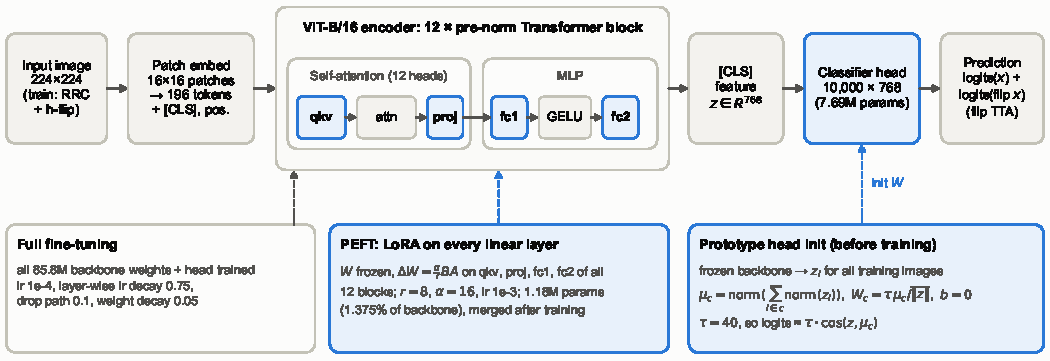
\includegraphics[width=\textwidth]{figures/fig0_framework.pdf}
  \caption{\textbf{Overview of our pipeline.}
  A ViT-B/16 backbone is adapted either by full fine-tuning or by LoRA on every linear layer (blue modules: qkv, proj, fc1, fc2 in all 12 blocks).
  Before training, the 10,000-way head is initialized by imprinting L2-normalized class-mean features (prototypes) with temperature $\tau$.
  At test time, the logits of the image and of its horizontal flip are summed.
  All runs use AdamW with warmup and cosine decay, bf16 and batch size 256, within a budget of 96\,GB$\cdot$h (1.2\,h on one A100-80GB).}
  \label{fig:framework}
\end{figure*}

\Cref{fig:framework} summarizes the pipeline.
Let $f_\theta$ map an image $x$ to its final-layer \texttt{[CLS]} feature $z = f_\theta(x) \in \mathbb{R}^{768}$, and let $h(z) = Wz + b$ with $W \in \mathbb{R}^{10000 \times 768}$ be the new classifier head.

\subsection{Backbone, budget and full fine-tuning}
\label{sec:budget}

\paragraph{Backbone.}
We use the timm~\cite{wightman2019timm} checkpoint \nolinkurl{vit_base_patch16_224.augreg2_in21k_ft_in1k}.
It is ViT-B/16 pretrained on ImageNet-21k with AugReg~\cite{steiner2022augreg} and fine-tuned on ImageNet-1k.
The backbone has 85,798,656 parameters; the 1,000-class head is replaced by a new 10,000-class head with 7,690,000 parameters.

\paragraph{Compute budget.}
The project allows 2\,h$\times$48\,GB $=$ 96\,GB$\cdot$h per training run ($\pm$10\%).
We convert this by the memory of the card we use: 1.2\,h on an 80\,GB A100.
Our clock counts everything that uses the GPU for training: head initialization (including feature extraction), all optimizer steps, and the holdout evaluation after every epoch.
It excludes unpacking the data, writing checkpoints and the final predictions.
After timing training steps 20--120, the cosine schedule is compressed if the planned number of epochs would exceed 97\% of the budget, and training stops at 1.05$\times$ the budget.
Every run reported here finished within 1.06 GPU-hours.

\paragraph{Full fine-tuning.}
All backbone and head weights are trained with AdamW~\cite{loshchilov2019adamw} at learning rate $10^{-4}$ and weight decay 0.05 (none on biases, normalization parameters, the class token and position embeddings).
We use layer-wise learning-rate decay of 0.75~\cite{bao2022beit} and drop path 0.1~\cite{huang2016stochastic}.
The learning rate warms up linearly (one epoch for runs of 6 or more epochs, 0.3 epochs for 3-epoch runs) and then follows a cosine decay to zero~\cite{loshchilov2017sgdr}.
Other settings are batch size 256, bf16 mixed precision, gradient clipping at norm 1, and label smoothing 0.1~\cite{szegedy2016rethinking}.
Training augmentation is RandomResizedCrop (scale 0.25--1) plus horizontal flip.
For evaluation, images are resized to 248 pixels and center-cropped to 224.

\subsection{Parameter-efficient adaptation}
\label{sec:peft}

\paragraph{LoRA.}
For a frozen linear layer $W_0 \in \mathbb{R}^{d_\text{out} \times d_\text{in}}$, LoRA~\cite{hu2022lora} computes
\begin{equation}
  y = W_0 x + \tfrac{\alpha}{r} B A x,
  \label{eq:lora}
\end{equation}
where $A \in \mathbb{R}^{r \times d_\text{in}}$ and $B \in \mathbb{R}^{d_\text{out} \times r}$ are trainable.
$B$ is initialized to zero, so training starts exactly from the pretrained model.
We use $r = 8$ and $\alpha = 16$.
timm fuses the query, key and value projections into a single \texttt{qkv} layer.
LoRA on \texttt{qkv} therefore adapts all three projections, with the same parameter count (294,912, 0.344\% of the backbone) as LoRA on separate query and value projections.
Our final PEFT variant applies LoRA to all four linear layers of every block (\texttt{qkv}, \texttt{proj}, \texttt{fc1}, \texttt{fc2}), for 1,179,648 parameters (1.375\%).
The LoRA weights and the head use learning rate $10^{-3}$ and weight decay $10^{-4}$, with no LoRA dropout.
After training, $\tfrac{\alpha}{r}BA$ is merged into $W_0$, so inference uses exactly the base architecture.

\paragraph{AdaptFormer.}
Following~\cite{chen2022adaptformer}, each block gains a bottleneck branch in parallel to its MLP:
\begin{equation}
  x_{l+1} = x' + \mathrm{MLP}(\mathrm{LN}(x')) + s \cdot W_\text{up}\,\mathrm{ReLU}(W_\text{down} x'),
  \label{eq:adaptformer}
\end{equation}
where $x'$ is the output of the attention sub-block.
We use bottleneck width 64, scale $s = 0.1$, dropout 0.1 and a zero-initialized $W_\text{up}$, for 1,189,632 parameters (1.387\%).
Unlike LoRA, the branch cannot be merged into the backbone.

In all PEFT runs the head is also trained.
Because the head alone has 7.69M parameters, we report trainable parameters both excluding it (the convention of the project's 0.34\% LoRA reference) and including it.

\subsection{Initializing the 10,000-way head}
\label{sec:head-init}

The head is the largest new component, and each of its rows sees at most 45 images.
A random head produces near-uniform logits (initial loss $\approx \ln 10000 = 9.2$), and the backbone receives large, noisy gradients from it early in training.
We compare three initializations.

\paragraph{Random.} timm's default initialization of a new linear layer.

\paragraph{Prototype (imprinted) head.}
With the frozen pretrained backbone, we extract features $z_i$ for all training images once.
We then imprint L2-normalized class means~\cite{snell2017prototypical,qi2018imprinted}:
\begin{equation}
  \mu_c = \frac{\sum_{i:\,y_i=c} \hat z_i}{\big\|\sum_{i:\,y_i=c} \hat z_i\big\|}, \quad
  W_c = \frac{\tau}{\overline{\|z\|}}\, \mu_c, \quad b_c = 0,
  \label{eq:proto}
\end{equation}
where $\hat z_i = z_i / \|z_i\|$ and $\overline{\|z\|}$ is the mean feature norm, so that logits are approximately $\tau \cos(z, \mu_c)$.
The temperature $\tau$ is chosen from $\{5, 10, 15, 20, 30, 40, 60, 80\}$ by the cross-entropy on 10,000 training features, which selects $\tau = 40$.
This head alone, with zero trainable parameters, reaches 44.0\% holdout accuracy.
Feature extraction takes 6--7 minutes on an A100, and this time is counted in every run's GPU-hours.

\paragraph{Linear-probe (LP) head.}
Starting from the prototype head, we train $(W, b)$ on the cached frozen features for 10 epochs.
We use AdamW (learning rate $10^{-3}$, weight decay $10^{-4}$), batch size 4,096, cosine decay and label smoothing 0.1.
This reaches 62.1\% holdout accuracy in a few seconds and corresponds to the first stage of LP-FT~\cite{kumar2022lpft}.
It was our initial design, chosen to avoid feature distortion from a random head.
\Cref{sec:ablation-head} shows that it is the worst of the three choices.

\subsection{Test-time augmentation}
Following common practice~\cite{krizhevsky2012imagenet}, we sum the logits of an image and its horizontal flip.
This doubles inference cost and is applied only where stated.
